\documentclass[11pt]{article}
\usepackage[margin=1in]{geometry}
\usepackage{graphicx}
\usepackage{booktabs}
\usepackage{amsmath}
\usepackage{caption}
\captionsetup{font=small,labelfont=bf}
\usepackage[colorlinks=true,citecolor=blue,linkcolor=blue,urlcolor=blue]{hyperref}

\title{Which ESM-2 layer should you feed a mutation-effect predictor?\\
A 33-layer $\times$ 4-protein audit}
\author{Cheng Ding$^{1,\ast}$\\
\small $^{1}$School of Life Science and Technology, ShanghaiTech University, Shanghai, China\\
\small $^{\ast}$Correspondence: \texttt{dingcheng2024@shanghaitech.edu.cn}; ORCID: \href{https://orcid.org/0009-0001-7221-9066}{0009-0001-7221-9066}}
\date{}

\begin{document}
\maketitle

\begin{abstract}
Supervised mutation-effect predictors built on protein language models (PLMs) inherit a
hidden degree of freedom: which transformer layer to read out. Probing studies in NLP and,
more recently, in protein modelling suggest that intermediate layers carry the most
structural and functional signal, while the final layers specialize toward the pre-training
objective. Whether this picture governs deep-mutational-scanning (DMS) prediction is rarely
tested directly; most pipelines simply default to the last layer. Here we audit the question
exhaustively on four DMS systems (SARS-CoV-2 RBD binding, caspase-3 activity, a TIM-barrel
fitness landscape, and the $\lambda$ cI repressor) by training matched probe heads on all 33
layers of ESM-2 (650M), under two architectures --- a single-stream baseline and a
two-stream cross-attention model that fuses each layer with an alignment-free structural
representation ($Z_{II}$, extracted from RoseTTAFold3) --- with paired splits and paired
initializations (33 layers $\times$ 3 splits $\times$ 2 seeds per cell). The optimal layer is
protein-specific: RBD peaks at layer 10 (Spearman $\rho$ 0.5141 versus 0.4536 at the last
layer), cI at layer 32, and TIM and caspase-3 at the last layer. Fusing a structural second
stream lifts accuracy but does not relocate the optimum (cross-layer correlation of the two
profiles $0.78$--$0.98$). The fusion gain is itself layer-structured, largest at early layers
and shrinking to below the $\pm 0.02$ reproducibility floor exactly where the PLM stream is
already strongest. Linear CKA between each ESM-2 layer and the structural representation
supports the ``intermediate layers encode structure'' picture on two proteins and inverts it
on the other two, and an effective-rank analysis shows the last-layer representation
collapses to roughly one quarter of the intrinsic dimensionality of the best intermediate
layer. We conclude that layer choice is a dataset-specific hyperparameter that should be
swept, not assumed, and we provide a cheap protocol for doing so.
\end{abstract}

\section{Introduction}

Protein language models (PLMs) trained on hundreds of millions of sequences produce
per-residue representations that transfer broadly to structure and function
prediction~\cite{rives2021,lin2023}. In supervised variant-effect prediction, the dominant
recipe is to freeze the PLM, read out one layer --- almost always the last --- and train a
small prediction head on top~\cite{notin2023}. The choice of layer is rarely discussed, yet
it is a genuine degree of freedom: a 33-layer model such as ESM-2 650M offers 33 materially
different representations of the same sequence. Two forces make the choice non-trivial. On
one hand, deeper layers integrate more context and approach the representation used for the
model's own pre-training predictions. On the other hand, the masked-modelling objective
shapes the final layers toward token reconstruction, not toward any particular downstream
quantity, so there is no guarantee that the last layer is the best read-out for a fitness
label.

A loose consensus from probing work suggests where the useful signal should sit. In NLP,
layer-wise probing showed that BERT's layers recapitulate a classical processing pipeline,
with syntactic structure concentrated in intermediate
layers~\cite{tenney2019}. Analyses of contextual embeddings further showed that final layers
are highly anisotropic and specialized to the training objective~\cite{ethayarajh2019}. For
PLMs specifically, recent geometric analyses report that structure-related signal peaks
before the final layer and that effective dimensionality contracts toward the output
layers~\cite{beshkov2025}. If this picture held universally for mutation-effect prediction,
practitioners could fix an intermediate layer once and for all. Whether it holds is an
empirical question, and it matters in practice: layer choice is made silently in every DMS
pipeline, costs nothing to sweep once features are cached, and interacts with a second
increasingly common design decision --- whether to fuse PLM embeddings with structure-based
representations.

We test this directly. Rather than probing for what a layer \emph{encodes}, we measure what
a layer \emph{affords}: we train identical supervised heads on each of the 33 layers of
ESM-2 650M across four deep-mutational-scanning (DMS) datasets spanning different proteins,
assays, and selection types, with position-held-out validation and paired seeds. We then
repeat the entire sweep in a two-stream architecture that fuses each layer with $Z_{II}$, an
alignment-free structural representation extracted from RoseTTAFold3 (RF3)~\cite{corley2025}.
This design answers three practical questions: (i) does the best layer coincide across
proteins; (ii) does adding structural information change which layer is best; and (iii)
where along the depth axis does a structural second stream actually add information? We
complement the supervised curves with layer-resolved representational-similarity (linear
CKA~\cite{kornblith2019}) and effective-rank measurements that connect the performance
profile to the geometry of the representations.

Throughout, we interpret differences against an empirically calibrated noise floor of
$\pm 0.02$ in validation Spearman $\rho$ (Methods), and we do not draw conclusions from
differences smaller than this floor.

\section{Results}

\subsection{The optimal ESM-2 layer is protein-specific}

Figure~\ref{fig:profiles} (grey curves) shows validation Spearman $\rho$ of single-stream
(SP) probe heads trained on each of the 33 ESM-2 layers for the four DMS systems, averaged
over 3 position-held-out splits $\times$ 2 initializations. The four profiles share no
common optimum (Table~\ref{tab:peaks}). RBD binding prediction peaks at layer~10
($\rho=0.5141$), exceeding the conventional last-layer choice by $+0.0605$ ($0.4536$ at
L33) --- three times the noise floor. The $\lambda$ cI repressor peaks at L32
($0.5416$ versus $0.5037$ at L33, $+0.0380$). In contrast, TIM-barrel fitness and caspase-3
activity are predicted best from the last layer ($0.5992$ and $0.5826$), and both profiles
rise essentially monotonically with depth. The peaks are robust to resampling: the
per-layer standard deviation across the six split $\times$ seed runs (median $0.026$--$0.061$
across proteins) reflects split heterogeneity more than run-to-run jitter, and the RBD and CI
peak-to-L33 gaps exceed it comfortably. Thus the ``intermediate layers are best''
expectation is confirmed in one system out of four, the ``last layer'' default is correct in
two, and one system prefers the penultimate layer. Neither of the two standard heuristics
--- always use the last layer, or always use a fixed intermediate layer --- is safe.

Beyond the peak positions, the profile \emph{shapes} differ qualitatively. RBD rises from
$0.366$ at L1 to a broad early plateau ($\approx 0.49$--$0.51$ over L5--L12) and then decays
monotonically to the last layer, losing $0.06$ from plateau to L33. CI, the smallest dataset
($N=351$) and the noisiest profile (median per-layer s.d.\ $0.061$), dips in the early-middle
layers ($0.285$ at L5) and climbs steeply from L15 ($0.459$) to its L32 peak before dropping
$0.038$ at L33. TIM and CASP3 both show poor early layers ($\approx 0.30$--$0.36$ through L8)
followed by an essentially monotone climb (TIM: $0.488$ at L10 to $0.599$ at L33; CASP3:
$0.421$ at L10 to $0.583$ at L33). The early-layer weakness of TIM and CASP3 foreshadows the
fusion result below: it is exactly these poorly performing layers that gain most from a
structural second stream.

\begin{figure}[t]
\centering
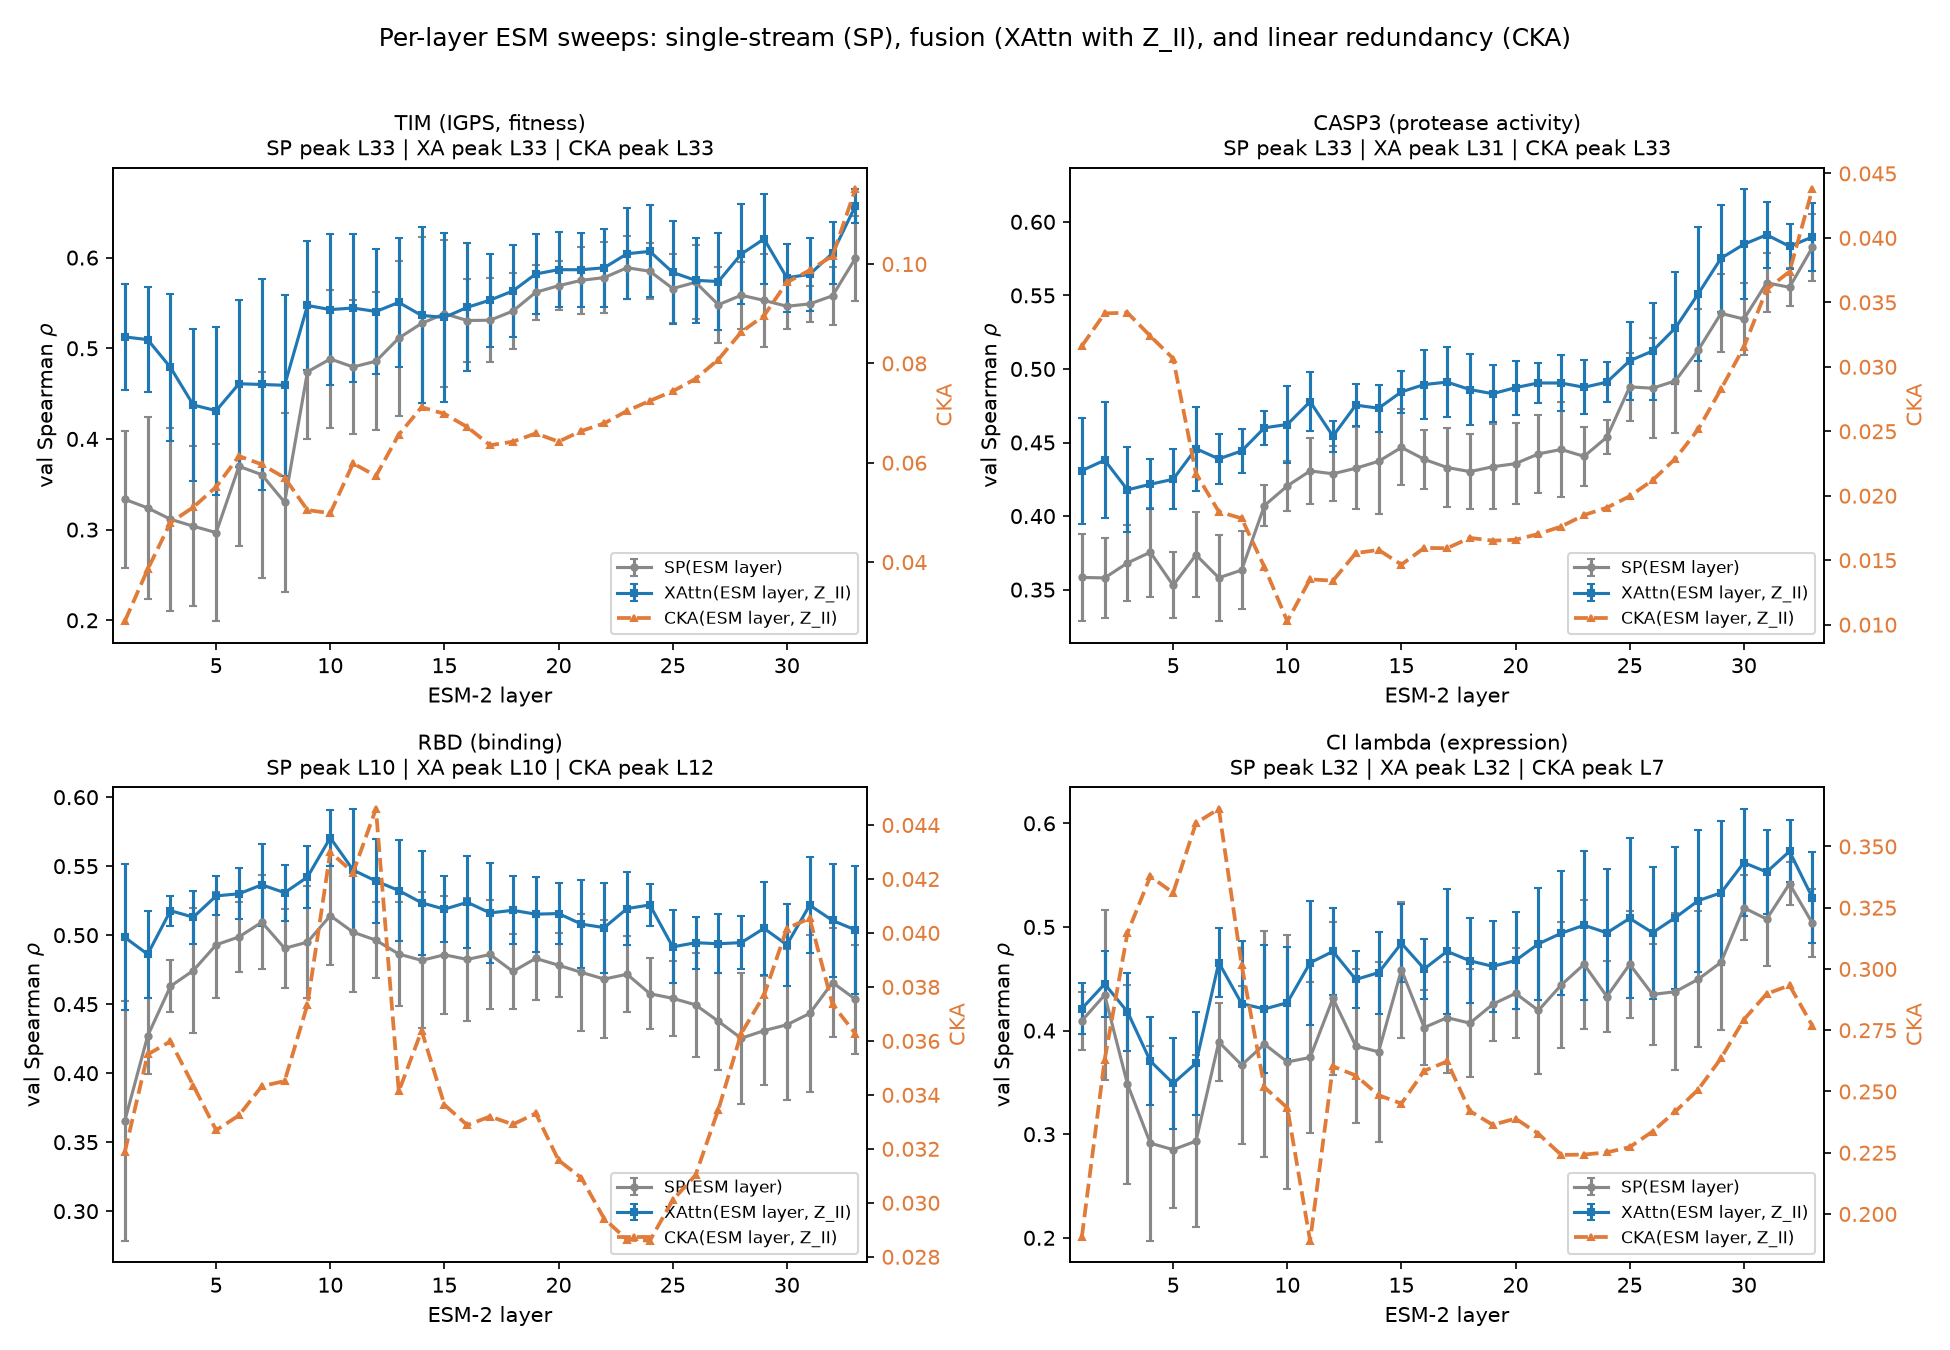
\includegraphics[width=\textwidth]{figures/fig1_layer_profiles.png}
\caption{\textbf{Per-layer ESM-2 sweeps on four DMS systems.} Grey: single-stream (SP)
probe validation Spearman $\rho$ per layer (mean over 3 position-held-out splits $\times$ 2
initializations; error bars $\pm 1$ s.d.). Blue: two-stream cross-attention fusion (XAttn)
of the same layer with $Z_{II}$. Orange dashed (right axis): linear CKA between the layer's
per-residue representation and $Z_{II}$. Panel headers report the peak layer of each curve.}
\label{fig:profiles}
\end{figure}

\begin{table}[t]
\centering
\small
\setlength{\tabcolsep}{4.5pt}
\caption{\textbf{Peak layers and last-layer baselines.} Mean validation Spearman $\rho$ (3
splits $\times$ 2 inits). SP = single-stream probe; XA = cross-attention fusion with
$Z_{II}$; marginal = XA $-$ SP at the SP-optimal layer. $\Delta_{\text{L33}}$ = SP best
$-$ SP L33. The $\pm 0.02$ noise floor applies to all differences.}
\label{tab:peaks}
\begin{tabular}{lcccccc}
\toprule
Protein & SP best (layer) & SP L33 & $\Delta_{\text{L33}}$ & XA best (layer) & XA L33 & marginal \\
\midrule
RBD   & 0.5141 (L10) & 0.4536 & $+0.0605$ & 0.5706 (L10) & 0.5038 & $+0.0565$ \\
CASP3 & 0.5826 (L33) & 0.5826 & $0$       & 0.5912 (L31) & 0.5897 & $+0.0071$ \\
TIM   & 0.5992 (L33) & 0.5992 & $0$       & 0.6568 (L33) & 0.6568 & $+0.0576$ \\
CI    & 0.5416 (L32) & 0.5037 & $+0.0380$ & 0.5729 (L32) & 0.5283 & $+0.0313$ \\
\bottomrule
\end{tabular}
\end{table}

\subsection{Fusing a structural second stream does not relocate the optimal layer}

Repeating the sweep with the XAttn fusion architecture (Fig.~\ref{fig:profiles}, blue
curves) lifts performance on every protein and nearly every layer: the fusion marginal is
positive on 131 of 132 protein $\times$ layer cells and exceeds the noise floor in 119 of
them. The fusion profiles nevertheless track the SP profiles closely: the per-layer Pearson
correlation between the SP and XAttn curves is $0.98$ (CASP3), $0.95$ (CI), $0.92$ (TIM),
and $0.78$ (RBD). Accordingly, the XA
optimum sits at the same layer as the SP optimum on RBD (L10), CI (L32), and TIM (L33), and
on CASP3 it moves from L33 to L31 by $+0.0015$ --- an order of magnitude below the noise
floor and therefore not a real relocation. Layer choice and the fusion decision are thus
approximately separable: structural context changes \emph{how well} a layer performs, not
\emph{which} layer is best.

\subsection{The fusion gain is layer-structured}

The per-layer fusion marginal (XA $-$ SP on identical splits and seeds;
Fig.~\ref{fig:marginal}) is far from constant (per-protein means $+0.047$ to $+0.057$), and
its shape is itself system-specific. On TIM it is U-shaped: $+0.179$ at L1,
decaying to $-0.004$ at L15 --- statistically indistinguishable from zero --- then
recovering to $+0.058$ at L33. On RBD the marginal is largest at L1 ($+0.133$) and re-rises
in deep layers (L31 $+0.079$) precisely where the SP profile decays, i.e.\ the structural
stream rescues degenerating layers. On CASP3 the marginal declines with depth and reaches
$+0.007$ at L33 --- below the noise floor, meaning the structural stream adds nothing at
CASP3's best layer. The pattern is consistent across systems: the second stream pays most
where the PLM stream is intrinsically weak, and least where it is already optimal. Notably,
the TIM marginal recovers at L33 exactly where ESM--$Z_{II}$ linear similarity is maximal
(Section~\ref{sec:cka}), so high linear redundancy does not imply uselessness: the fused
model still extracts non-linearly complementary signal there.

\begin{figure}[t]
\centering
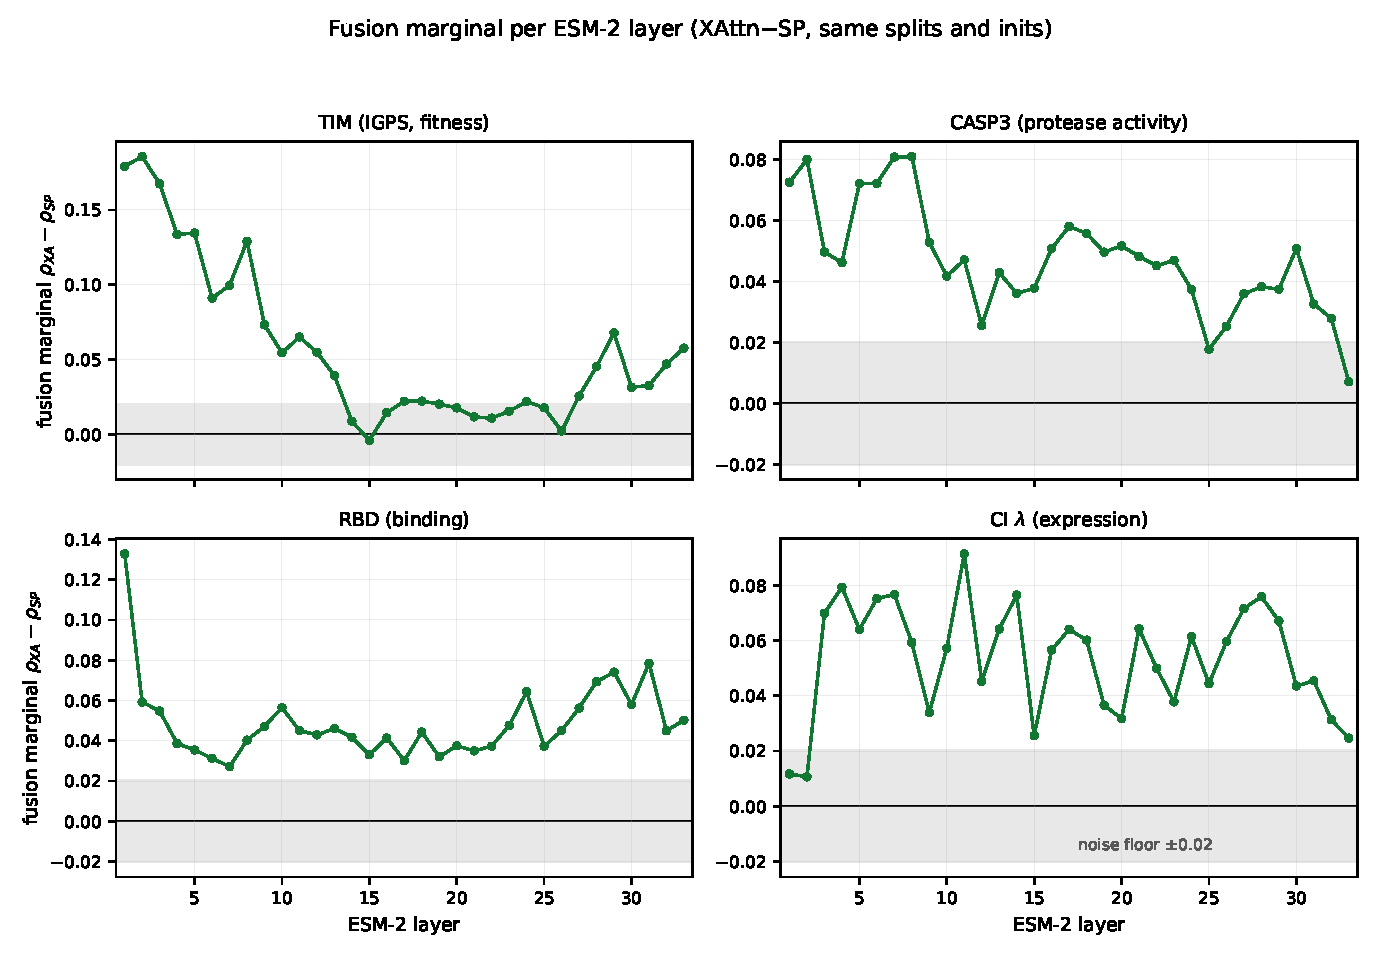
\includegraphics[width=\textwidth]{figures/fig2_fusion_marginal.pdf}
\caption{\textbf{Fusion marginal per layer} (XAttn $-$ SP, paired splits and seeds). The
shaded band marks the $\pm 0.02$ reproducibility floor: marginals inside it (e.g.\ CASP3 at
L33, TIM near L15) are treated as zero.}
\label{fig:marginal}
\end{figure}

\subsection{Representational similarity to structure: the literature picture holds in half
the systems}\label{sec:cka}

To relate these performance profiles to the ``intermediate layers encode structure''
hypothesis, we measured linear CKA between each layer's per-residue representation and the
$Z_{II}$ structural representation (Fig.~\ref{fig:profiles}, orange curves). RBD conforms to
the expected picture: CKA peaks at L12 ($0.0446$), adjacent to the SP performance peak at
L10. CI also peaks early (L7, $0.365$; we caution that the CI $Z_{II}$ extraction carries a
known indexing artifact, Methods). The other two systems invert the picture: TIM's CKA rises
monotonically to its maximum at L33 ($0.115$), and CASP3's is U-shaped with a minimum at
L9--15 ($\approx 0.010$) and its maximum, again, at L33 ($0.0438$). Consistent with this
split, the rank correlation between per-layer CKA and per-layer SP performance is strongly
positive on TIM ($\rho_s=+0.78$) and weak or negative elsewhere (CASP3 $+0.22$, RBD $+0.14$,
CI $-0.22$). Structural alignment of intermediate layers is therefore a system-dependent
property, not a universal feature of ESM-2 depth: the geometry that a probing study extracts
from one protein family does not transfer as a rule to another.

\subsection{Mechanistic clue: the last layer is intrinsically low-rank}\label{sec:rank}

Why would L10 outperform L33 on RBD? A per-representation effective-rank analysis
(Fig.~\ref{fig:rank}) shows that the RBD last-layer representation occupies far fewer
directions than the best intermediate layer: participation ratio $44.5$ at L33 versus
$205.7$ at L12 ($4.6\times$), and $325$ versus $702$ singular values needed for 90\% of
variance. An independent probe comparison on RBD confirms that the difference is not an
artifact of the main sweep: L12 scores $0.4955$ against L33's $0.4821$ under a matched
protocol. This is consistent with reports that final layers of masked language models
specialize toward the pre-training objective and become
anisotropic~\cite{ethayarajh2019,beshkov2025}: on systems where the assay rewards
structure-shaped intermediate features, the collapsed final layer is simply the wrong
read-out. We stress that this contraction is a property of the representation, not of the
label: TIM and CASP3 achieve their best $\rho$ on exactly this low-rank L33 read-out.

\begin{figure}[t]
\centering
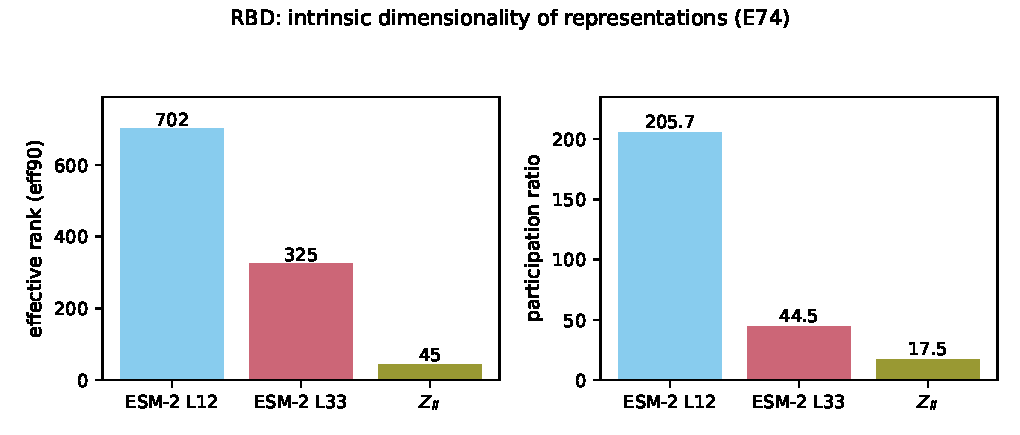
\includegraphics[width=0.85\textwidth]{figures/fig3_effective_rank.pdf}
\caption{\textbf{Intrinsic dimensionality of RBD representations.} Effective rank (left:
number of singular values capturing 90\% of variance; right: participation ratio) of ESM-2
L12, ESM-2 L33, and $Z_{II}$, computed over per-residue vectors.}
\label{fig:rank}
\end{figure}

\section{Discussion}

Our audit yields a simple practical message: the ESM-2 layer fed to a mutation-effect
predictor is a dataset-specific hyperparameter, and both popular defaults fail somewhere.
``Always use the last layer'' forfeits $+0.06$ Spearman on RBD and $+0.04$ on CI; ``use a
fixed intermediate layer'' forfeits the monotonic gains on TIM and CASP3. The remedy is
cheap. Because all 33 layers come out of a single forward pass, the sweep costs one feature
extraction plus $33 \times 6$ short head-trainings on frozen embeddings --- minutes per
layer on a single consumer GPU at our dataset sizes, orders of magnitude less than any
fine-tuning step. We therefore recommend a single-stream coarse sweep over all layers as a
standard first step in DMS pipelines, with the winner confirmed under the intended final
architecture. Two softer conclusions qualify the fusion literature. First, an auxiliary
structural stream does not relocate the optimal PLM layer, so layer selection and multimodal
design can be tuned independently. Second, the value of an auxiliary stream is predictable
in sign and rough location from the single-stream profile itself: it pays where the PLM
representation is poor (early layers, or deep layers whose single-stream performance has
decayed) and vanishes --- below a $\pm 0.02$ reproducibility floor --- where the PLM is
already at its best. Practitioners fusing structure with PLM features should therefore not
expect uniform additive gains across depths, and a single-layer fusion benchmark can
misrepresent what fusion offers at other depths.

Our results also draw a line between two questions that are easy to conflate. Probing studies
ask which layers \emph{contain} structure- or function-related signal, typically with linear
read-outs and information-theoretic controls; our audit asks which layer \emph{serves} a
supervised mutation-effect head trained under a realistic protocol. The two need not agree,
and on TIM and CASP3 they visibly do not: the layers most linearly aligned with a structural
representation are also the deepest, and there a linear notion of redundancy understates what
a nonlinear fusion head can still extract. Where they do agree (RBD, and partially CI), the
agreement is close enough to be practically useful --- the CKA peak sits within two layers of
the performance peak --- which suggests that a cheap representational screen can shortlist
candidate layers before any supervised sweep, but cannot replace it.

\paragraph{Limitations.} Four proteins and one model scale (ESM-2 650M) cannot support
universal claims; the split we observe (one mid-layer, one penultimate, two last-layer
optima) is a sample, not a taxonomy, and the optimum may shift with model size, probe
capacity, or metric (we used Spearman $\rho$ throughout). CKA is a linear similarity measure
and, as the TIM L33 result shows, underestimates non-linear complementarity. The CI $Z_{II}$
stream carries a known extraction artifact (Methods), so its absolute CKA values should be
read with caution. Our noise floor was calibrated on this pipeline's hardware and protocol;
other stacks should re-derive it. Finally, our study is silent on zero-shot scoring, where
the pre-training objective directly defines the read-out and different considerations apply.

\section{Methods}

\subsection{Datasets}

Four single-point DMS datasets were used (Table~\ref{tab:data}): SARS-CoV-2 RBD
(ACE2-binding affinity, \texttt{bind\_avg})~\cite{starr2020}; human caspase-3 (CASP3)
fluorescence activity~\cite{roychowdhury2022}, restricted to the 244-chain positions as in
the source pipeline; the \emph{Thermus thermophilus} TrpC TIM barrel
(organismal fitness; ProteinGym \texttt{TRPC\_THEMA\_Chan\_2017})~\cite{chan2017,notin2023};
and the $\lambda$ cI repressor high-expression assay (ProteinGym
\texttt{RPC1\_LAMBD\_Li\_2019\_high-expression})~\cite{li2019,notin2023}. Labels were
z-scored within each dataset.

\begin{table}[t]
\centering
\small
\setlength{\tabcolsep}{4.5pt}
\caption{\textbf{Datasets.} $N$ = number of mutants scored; positions = unique mutated
positions used for position-held-out splitting.}
\label{tab:data}
\footnotesize
\begin{tabular}{llcccl}
\toprule
System & Assay & $N$ & Positions & Length & Source \\
\midrule
RBD   & ACE2 binding        & 3998 & 201 & 201 & Starr et al.\ 2020~\cite{starr2020} \\
CASP3 & Protease activity   & 1469 & 244 & 244 (homo\-dimer 488) & Roychowdhury \& Romero 2022~\cite{roychowdhury2022} \\
TIM   & Organismal fitness  & 1519 & 80  & 254 & Chan et al.\ 2017~\cite{chan2017} \\
CI    & Expression (FACS)   & 351  & 59  & 237 & Li et al.\ 2019~\cite{li2019} \\
\bottomrule
\end{tabular}
\end{table}

\subsection{Representations}

For every mutant we ran a single-sequence forward pass of ESM-2 650M
(\texttt{esm2\_t33\_650M\_UR50D})~\cite{lin2023} and stored all 33 transformer-layer hidden
states as $[L,1280]$ tensors (per-mutant, not mutation-delta). The structural stream
$Z_{II}$ is the 128-dimensional pair representation of RoseTTAFold3 extracted without any
MSA input~\cite{corley2025}, used as per-residue row slices (RBD/TIM: row grid; CASP3: the
mutated row of the $488\times488$ homodimer pair block, first monomer). The CI $Z_{II}$
extraction uses a legacy indexing convention that is semantically offset but numerically
close to the corrected version (project audit: corrected-vs-artifacted baselines differ by
$\approx 0.01$); we flag all CI CKA values accordingly.

\subsection{Probe heads and training}

The single-stream (SP) head is a small transformer probe: Linear $1280\!\to\!256$,
sinusoidal positional encoding, a 3-layer Transformer encoder (8 heads, feed-forward 1024,
dropout 0.1), an output MLP ($256\!\to\!512\!\to\!128$), attention pooling over residues,
and a final MLP ($128\!\to\!64\!\to\!1$). The fusion (XAttn) head encodes each modality with
such an encoder ($\to128$ dimensions), applies a per-residue symmetric 2-token
cross-attention (1 layer, 4 heads) between the ESM and $Z_{II}$ token at each position,
concatenates the streams ($[L,256]$), and passes them through a 2-layer joint Transformer
(8 heads), attention pooling, and an MLP ($256\!\to\!128\!\to\!1$). PLM and RF3 weights are
frozen; only heads train.

Inputs are standardized per position and per channel (z-score over training samples), which
we found mandatory to preserve the ESM channel-variance hierarchy. Splits hold out 30\% of
mutated \emph{positions} (not mutants) to prevent positional leakage; three split seeds
(42--44) and two weight initializations (7, 107) give 6 runs per layer per architecture,
shared and paired between SP and XAttn. Training: 250 epochs, AdamW (lr $10^{-4}$, weight
decay 0.05), cosine schedule, batch size 128 (32 for CI), MSE loss on z-scored labels. The
reported metric is best-epoch validation Spearman $\rho$.

\subsection{Noise floor}

Identical cells re-run across processes and GPUs in this pipeline differ by up to
$0.021$ in validation $\rho$; we therefore adopt $\pm 0.02$ as a reproducibility floor and
treat any difference inside it as null. This floor is stated a priori and applied uniformly,
including to our own preferred narratives (e.g.\ the CASP3 L33 fusion marginal $+0.007$ is
reported as zero).

\subsection{Representational analyses}

Linear CKA~\cite{kornblith2019} between each ESM-2 layer and $Z_{II}$ was computed on
subsampled (mutant, position) pairs ($\leq 300$ mutants $\times$ 20 positions per mutant),
alongside ridge-regression $R^2$ (ESM $\to Z_{II}$, 80/20 split, $\lambda=100$). Effective
rank was measured on the covariance of per-residue vectors as (i) the number of singular
values capturing 90\% of total variance (eff90) and (ii) the participation ratio
$(\sum_i \lambda_i)^2 / \sum_i \lambda_i^2$.

\subsection*{Data availability}

All sweep results are archived as per-protein JSON result files from the four experiment
series underlying this study (E74, E75, E75b, E77); every number quoted in the text is
mapped to its source file in the accompanying \texttt{TRACEABILITY.md}. Analysis scripts
and all archived results are publicly available at
\url{https://github.com/Lizon1c/esm2-layer-audit-dms}.

\begin{thebibliography}{12}
\bibitem{rives2021}
Rives A, Meier J, Sercu T, Goyal S, Lin Z, Liu J, et al.
Biological structure and function emerge from scaling unsupervised learning to 250 million
protein sequences. \emph{Proc Natl Acad Sci USA}. 2021;118(15):e2016239118.
doi:10.1073/pnas.2016239118.

\bibitem{lin2023}
Lin Z, Akin H, Rao R, Hie B, Zhu Z, Lu W, et al.
Evolutionary-scale prediction of atomic-level protein structure with a language model.
\emph{Science}. 2023;379(6637):1123--1130. doi:10.1126/science.ade2574.

\bibitem{notin2023}
Notin P, Kollasch A, Ritter D, van Niekerk L, Paul S, Spinner H, et al.
ProteinGym: Large-scale benchmarks for protein fitness prediction and design.
In: \emph{Advances in Neural Information Processing Systems}. Vol.~36; 2023. p.~64331--64379.

\bibitem{tenney2019}
Tenney I, Das D, Pavlick E.
BERT rediscovers the classical NLP pipeline.
In: \emph{Proceedings of the 57th Annual Meeting of the Association for Computational
Linguistics}; 2019. p.~4593--4601. doi:10.18653/v1/P19-1452.

\bibitem{ethayarajh2019}
Ethayarajh K.
How contextual are contextualized word representations? Comparing the geometry of BERT,
ELMo, and GPT-2 embeddings.
In: \emph{Proceedings of EMNLP-IJCNLP}; 2019. p.~55--65. doi:10.18653/v1/D19-1006.

\bibitem{beshkov2025}
Beshkov K, Malthe-S{\o}renssen A.
Towards understanding the shape of representations in protein language models.
\emph{arXiv:2509.24895}. 2025.

\bibitem{kornblith2019}
Kornblith S, Norouzi M, Lee H, Hinton G.
Similarity of neural network representations revisited.
In: \emph{Proceedings of the 36th International Conference on Machine Learning (PMLR 97)};
2019. p.~3519--3529.

\bibitem{corley2025}
Corley N, Butterfoss GL, Krishna R, et al.
Accelerating biomolecular modeling with AtomWorks and RF3.
\emph{bioRxiv}. 2025:2025.08.14.670328. doi:10.1101/2025.08.14.670328.

\bibitem{starr2020}
Starr TN, Greaney AJ, Hilton SK, Ellis D, Crawford KHD, Dingens AS, et al.
Deep mutational scanning of SARS-CoV-2 receptor binding domain reveals constraints on
folding and ACE2 binding. \emph{Cell}. 2020;182(5):1295--1310.e20.
doi:10.1016/j.cell.2020.08.012.

\bibitem{roychowdhury2022}
Roychowdhury H, Romero PA.
Microfluidic deep mutational scanning of the human executioner caspases reveals differences
in structure and regulation. \emph{Cell Death Discovery}. 2022;8:7.
doi:10.1038/s41420-021-00799-0.

\bibitem{chan2017}
Chan YH, Venev SV, Zeldovich KB, Matthews CR.
Correlation of fitness landscapes from three orthologous TIM barrels originates from
sequence and structure constraints. \emph{Nat Commun}. 2017;8:14614.
doi:10.1038/ncomms14614.

\bibitem{li2019}
Li X, Lalic J, Baeza-Centurion P, Dhar R, Lehner B.
Changes in gene expression predictably shift and switch genetic interactions.
\emph{Nat Commun}. 2019;10:3886. doi:10.1038/s41467-019-11735-3.
\end{thebibliography}

\end{document}
